% Template:     Template Reporte LaTeX
% Documento:    Archivo principal
% Versión:      2.0.5 (07/10/2020)
% Codificación: UTF-8
%
% Autor: Pablo Pizarro R.
%        Facultad de Ciencias Físicas y Matemáticas
%        Universidad de Chile
%        pablo@ppizarror.com
%
% Sitio web:    [https://latex.ppizarror.com/reporte]
% Licencia MIT: [https://opensource.org/licenses/MIT]

% CREACIÓN DEL DOCUMENTO
\documentclass[letterpaper,oneside]{article}

% INFORMACIÓN DEL DOCUMENTO
\def\titulodelreporte {CC3501: Tarea 1C - Snake}
\def\temaatratar {Snake}
\def\fechadelreporte {\today}

\def\autordeldocumento {Camilo Núñez Barra}
\def\nombredelcurso {Curso}
\def\codigodelcurso {CC3501-1}

\def\nombreuniversidad {Universidad de Chile}
\def\nombrefacultad {Facultad de Ciencias Físicas y Matemáticas}
\def\departamentouniversidad {Departamento de Ciencias de la Computación}
\def\imagendepartamento {departamentos/dcc}
\def\localizacionuniversidad {Santiago, Chile}

% IMPORTACIÓN DEL TEMPLATE
\input{template}
\usepackage{tikz}
\usetikzlibrary{shapes.multipart}
\usetikzlibrary{positioning}
\usetikzlibrary{decorations.text}
\usepackage{dirtree}

% INICIO DE PÁGINAS
\begin{document}
	
% CONFIGURACIÓN DE PÁGINA Y ENCABEZADOS
\templatePagecfg

% CONFIGURACIONES FINALES
\templateFinalcfg

% ======================= INICIO DEL DOCUMENTO =======================

% Título y nombre del autor
\inserttitle

% Resumen o Abstract
\begin{abstract}

Una serpiente con hambre infinita de manzanas crece cada vez que come una. La serpiente muere al tocarse a sí misma o al tocar uno de los bordes del mapa en el cual se mueve. Se implementa el patrón de arquitectura de software Modelo--Vista--Controlador, permitiendo al usuario definir el mapa sobre el que la serpiente, modelada como una matriz de tiempos, puede visualizarse en dos dimensiones, mediante la interfaz gráfica de PyOpenGL y GLFW.

\end{abstract}

% Ejemplo, se puede borrar
% \input{example}
\section{Solución propuesta}

Se utiliza el patrón de arquitectura de software Modelo--Vista--Controlador, de modo que el usuario, al interactuar con la interfaz de GLFW, usa el controlador mediante ciertas teclas, que manipulan los modelos de PyOpenGL, actualizando la vista del usuario y generando así un bucle de interacción que permite la ejecución del juego. El diagrama de este patrón se muestra en la figura \ref{fig:mvc}.

La serpiente tiene un valor propio de tiempo, que cuenta la cantidad de fotogramas ya mostrados, además, la cabeza avanza una casilla en cada fotograma, según la dirección indicada por el controlador. La serpiente se modela como una matriz de tiempos del tamaño de la grilla del mapa, y que se inicializa con valores \texttt{-1}. Sea \texttt{t} el número actual de fotogramas y \texttt{(x,y)} las coordenadas de la posición actual de la cabeza de la serpiente, entonces se asigna \texttt{matriz[y][x]=t} para cada iteración. La serpiente tiene largo de valor \texttt{L}, que corresponde a la cantidad de manzanas comidas más uno. Luego, solamente se dibujan las partes de la serpiente, mediante texturas, tales que sus coordenadas \texttt{(x,y)} cumplen con \texttt{t-matriz[y][x]<L}.

Si las coordenadas de la posición de la manzana, que se modela con primitivas de PyOpenGL, coinciden con las coordenadas de la posición de la cabeza de la serpiente, entonces se aumenta el largo en uno y la manzana reaparece en una posición que no contenga una parte de la serpiente.

Si la cabeza tiene una posición fuera de la grilla, y, por lo tanto inválida, la serpiente muere, así mismo si la cabeza coincide con una parte de la serpiente.

\section{Instrucciones de ejecución}
\begin{enumerate}
	\item Descargar Python 3.8.5 de \url{https://www.python.org/downloads/release/python-385/} e instalar, añadiendo al PATH.
	
	\item Descargar la carpeta \texttt{tarea1c} de \url{https://github.com/camilo-nb/CC3501-tareas}. La estructura de esta carpeta se muestra en la figura \ref{fig:dir}.
	
	\item Abrir el intérprete de comandos en la carpeta \texttt{tarea1c}. Por ejemplo, en Microsoft Windows se puede usar \texttt{cmd.exe}.
	
	\item Instalar las librerías: \texttt{glfw==1.12.0}, \texttt{PyOpenGL==3.1.5} y \texttt{numpy==1.19.1}, mediante el comando \texttt{pip install -r requirements.txt}.
	
	\item Ejecutar el código de la tarea, mediante el comando \texttt{python main.py [options]}. La lista completa de comandos de opciones está disponible en la tabla \ref{tab:cmd}. Ingresar (obligatoriamente) el tamaño \texttt{N} de la grilla cuadrada con \texttt{-n N}. Por ejemplo, se puede ejecutar \texttt{python main.py -n 50 -w 1280 -h 720 -f 24 -s off}, para una grilla cuadrada de $50\times50$, ventana de $1280\times720$ píxeles de resolución, velocidad de 24 fotogramas por segundos y sonido desactivado.
	
	\item Usar las teclas de movimiento: \texttt{W} arriba, \texttt{A} izquierda, \texttt{S} abajo y \texttt{D} derecha, con el objetivo de que la serpiente alcance la manzana. Se pierde al tocar el borde del mapa o al comerse a sí misma, de modo que aparece la escena final, activando las teclas: \texttt{F} rendirse y \texttt{R} reiniciar.
\end{enumerate}


\section{Resultados}

La figura \ref{fig:cmd} muestra la penúltima instrucción de ejecución, que permite crear una ventana, mostrando luego el juego, como, por ejemplo, la ventana que aparece en la figura \ref{fig:snake} (los comandos de opciones para ambas figuras son diferentes), que tiene una serpiente de largo 9 y un usuario cuyos últimos tecleos fueron \texttt{W}, \texttt{A}, y \texttt{W}. El usuario eventualmente pierde y se despliega la escena final de la figura \ref{fig:gameover}. El video de demostración se puede ver en \url{https://youtu.be/6lD3HlsB56Q}.

\section*{Anexo}

\begin{figure}[H]
	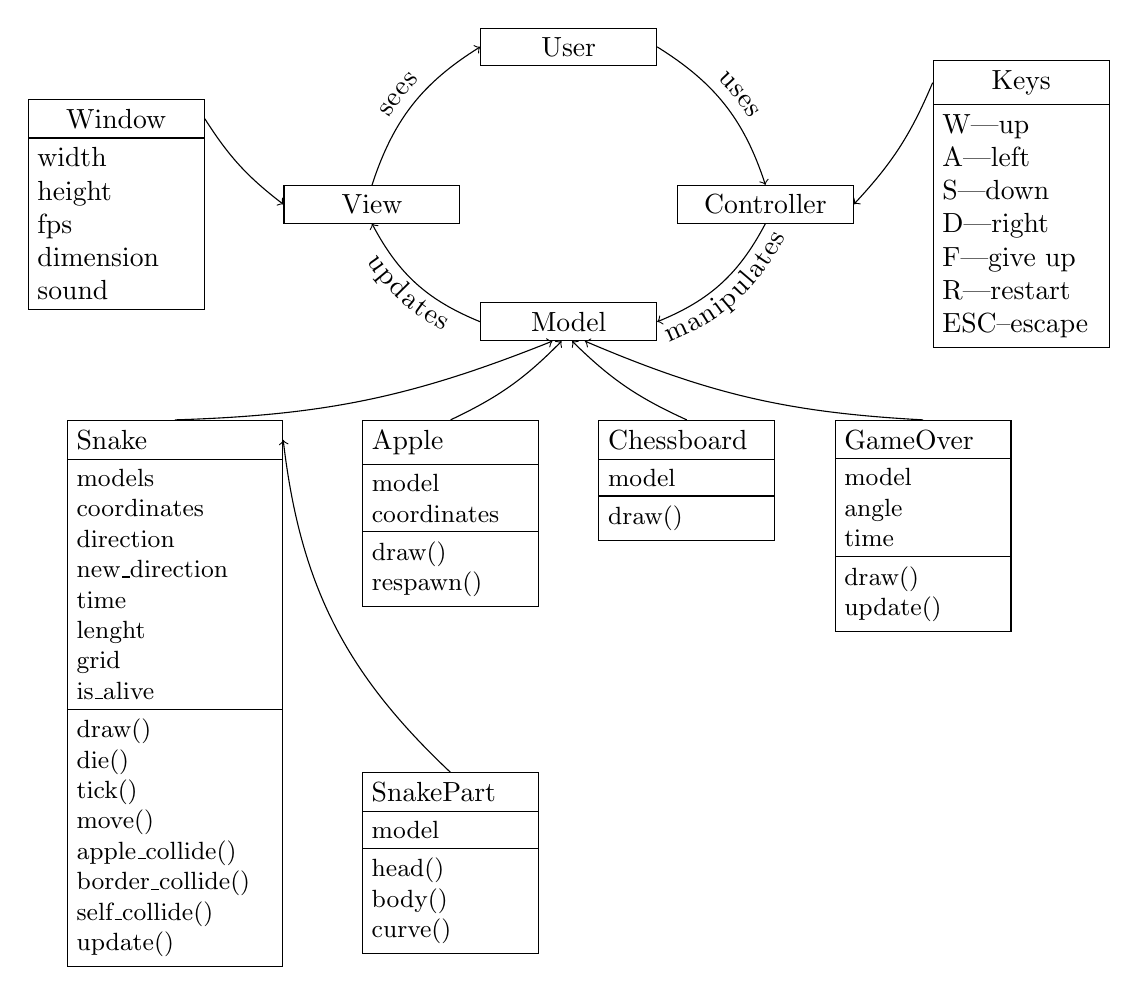
\begin{tikzpicture}[
		myrect/.style={
			rectangle split,
			rectangle split parts=3,
			draw,
			anchor=center
			every text node part/.style={align=center},
			every two node part/.style={font={\small}},
			every three node part/.style={font={\small}},
			text width=2cm
		}
		]
		
		\node[
		shape=rectangle,
		draw,
		text width=2cm,
		align=center
		] (model) {Model};
		
		\node[
		shape=rectangle,
		draw,
		above right=of model,
		text width=2cm,
		align=center,
		xshift=-0.75cm
		] (controller) {Controller};
		
		\node[
		rectangle split,
		rectangle split parts=2,
		draw,
		right=of controller,
		text width=2cm,
		every text node part/.style={align=center}
		] (keys) 
		{
			Keys
			\nodepart{two}
			W---up \\
			A---left\\
			S---down\\
			D---right\\
			F---give up\\
			R---restart\\
			ESC--escape
		};
		
		\node[
		shape=rectangle,
		draw,
		above left=of model,
		text width=2cm,
		align=center,
		xshift=0.75cm
		] (view) {View};
		
		\node[
		rectangle split,
		rectangle split parts=2,
		draw,
		left=of view,
		text width=2cm,
		every text node part/.style={align=center}
		] (window)
		{
			Window
			\nodepart{two}
			width \\
			height \\
			fps \\
			dimension \\
			sound
		};
		
		\node[
		shape=rectangle,
		draw,
		above=3cm of model,
		text width=2cm,
		align=center
		] (user) {User};
		
		\node[myrect, text width=2.5cm, below=of model, xshift=-5cm] (snake)
		{Snake
			\nodepart{two}
			models \\
			coordinates \\
			direction \\
			new\_direction \\
			time \\
			lenght \\
			grid \\
			is\_alive
			\nodepart{three}
			draw() \\
			die() \\
			tick() \\
			move() \\
			apple\_collide() \\
			border\_collide() \\
			self\_collide() \\
			update()};
		
		\node[myrect, below right=of snake.east] (snakepart)
		{SnakePart
			\nodepart{two}
			model
			\nodepart{three}
			head() \\
			body() \\
			curve()};
		
		\node[myrect, below=of model, xshift=-1.5cm] (apple)
		{Apple
			\nodepart{two}
			model \\
			coordinates
			\nodepart{three}
			draw() \\
			respawn()};
		
		\node[myrect, below=of model, xshift=1.5cm] (chessboard)
		{Chessboard
			\nodepart{two}
			model
			\nodepart{three}
			draw()};
		
		\node[myrect, below=of model, xshift=4.5cm] (gameover)
		{GameOver
			\nodepart{two}
			model \\
			angle \\
			time
			\nodepart{three}
			draw() \\
			update()};
		
		%%%%%%%%%%
		
		\draw[->, bend left=20] (snakepart.north) to (snake.text east);
		
		\draw[->, bend right=10] (snake.north) to (model.230);
		\draw[->, bend right=10] (apple.north) to (model.250);
		\draw[->, bend left=10] (chessboard.north) to (model.280);
		\draw[->, bend left=10] (gameover.north) to (model.310);
		
		\draw[<-,postaction={decorate,decoration={raise=-2ex,text along path,text align=center, text={updates}}}] (view.south) to [bend right=20] (model.west);
		
		\draw[<-,postaction={decorate,decoration={raise=-2ex,text along path,text align=center, text={manipulates}}}] (model.east) to [bend right=20] (controller.south);
		
		\draw[->,postaction={decorate,decoration={raise=1ex,text along path,text align=center, text={uses}}}] (user.east) to [bend left=20] (controller.north);
		
		\draw[->,postaction={decorate,decoration={raise=1ex,text along path,text align=center, text={sees}}}] (view.north) to [bend left=20] (user.west);
		
		\draw[->, bend left=10] (keys.text west) to (controller.east);
		
		\draw[->, bend right=10] (window.text east) to (view.west);
		
		
	\end{tikzpicture}
	\caption{Patrón Modelo--Vista--Controlador}
	\label{fig:mvc}
\end{figure}

\begin{figure}[H]
	\begin{minipage}{2in}
		\dirtree{%
			.1 tarea1c/.
			.2 controller/.
			.3 controller.py.
			.2 data/.
			.3 data.json.
			.3 doh.mp3.
			.3 hola.mp3.
			.3 mmm.mp3.
			.3 mydata.py.
			.2 lib/.
			.3 basic\_shapes.py.
			.3 easy\_shaders.py.
			.3 playsound.py.
			.3 scene\_graph.py.
			.3 transformations.py.
			.2 model/.
			.3 actor/.
			.4 body.png.
			.4 body\_tail.png.
			.4 curve.png.
			.4 green.png.
			.4 head\_0.png.
			.4 head\_1.png.
			.4 head\_2.png.
			.4 head\_3.png.
			.4 snake.py.
			.3 apple.py.
			.3 chessboard.py.
			.3 gameover.png.
			.3 gameover.py.
			.3 models.py.
			.2 view/.
			.3 view.py.
			.2 demo.mp4.
			.2 main.py.
			.2 reporte.pdf.
			.2 requirements.txt.
		}
	\end{minipage}
	\caption{Estructura de la carpeta \texttt{tarea1c}}
	\label{fig:dir}
\end{figure}

\begin{table}[H]
	\centering
	\begin{tabular}{|lcllc|}
		\hline
		
		comando & valor & descripción & tipo & por defecto\\
		
		\hline
		
		\texttt{-n}, \texttt{-{}-dimension} & int &
		\begin{tabular}[l]{@{}l@{}}Dimensiones del mapa\\ (grilla cuadrada)\end{tabular}
		& requerido & ---\\
		
		\hline
		
		\texttt{-w}, \texttt{-{}-width} & int &
		\begin{tabular}[l]{@{}l@{}}Ancho de la ventana\\ (pixeles)\end{tabular}
		& opcional & \texttt{800}\\
		
		\hline	
		
		\texttt{-h}, \texttt{-{}-height} & int &
		\begin{tabular}[l]{@{}l@{}}Alto de la ventana\\ (pixeles)\end{tabular}
		& opcional & \texttt{600}\\
		
		\hline
		
		\texttt{-f}, \texttt{-{}-fps} & int &
		\begin{tabular}[l]{@{}l@{}}Fotogramas por segundo\\ (velocidad)\end{tabular}
		& opcional & \texttt{10}\\
		
		\hline
		
		\texttt{-s}, \texttt{-{}-sound} & on/off &
		Música y efectos especiales
		& opcional & \texttt{on}\\
		
		\hline
	\end{tabular}
	\caption{Comandos de opciones}
	\label{tab:cmd}
\end{table}

\begin{figure}[H]
	\includegraphics[width=3in]{cmd.png}
	\caption{Ejecución del código en el intérprete de comandos}
	\label{fig:cmd}
\end{figure}

\begin{figure}[H]
	\includegraphics[width=3in]{snake.png}
	\caption{Snake a punto de comer una manzana, en una grilla de tamaño 10}
	\label{fig:snake}
\end{figure}

\begin{figure}[H]
	\includegraphics[width=3in]{gameover.png}
	\caption{Escena final}
	\label{fig:gameover}
\end{figure}


% FIN DEL DOCUMENTO
\end{document}
